\documentclass[a4paper,11pt,french]{article}
\usepackage[utf8]{inputenc}

\usepackage[T1]{fontenc}
\usepackage[francais]{babel} 
\usepackage[top=2cm, bottom=2cm, left=2cm, right=2cm, includeheadfoot]{geometry} %pour les marges
\usepackage{lmodern}
\usepackage{pict2e}
\usepackage{tikz}	
\usepackage{tikz-uml}
\usepackage{fancyhdr} % Required for custom headers
\usepackage{lastpage} % Required to determine the last page for the footer
\usepackage{extramarks} % Required for headers and footers
\usepackage{graphicx} % Required to insert images
\usepackage{tabularx, longtable}
\usepackage{color, colortbl}
\usepackage{lscape}
\usepackage[hidelinks]{hyperref}
\usepackage{longtable}
\usepackage{multirow}
\usepackage{rotating}
\usepackage{pgfgantt}
\usepackage{pgfcalendar}
\usepackage{ifthen}
\usepackage{gensymb}
\usepgflibrary{arrows} % for pgf-umlsd

\usetikzlibrary{trees,shapes.geometric,arrows,decorations.pathmorphing,backgrounds,fit,positioning,shapes.symbols,chains	}

\linespread{1.1} % Line spacing

% Set up the header and footer
\pagestyle{fancy}
\lhead{\textbf{\hmwkClass -- \hmwkSubject \\ \hmwkTitle \\ \hmwkDocName}} % Top left header
\rhead{
\includegraphics[width=10em]{logo_univ.png}}
\lfoot{\lastxmark} % Bottom left footer
\cfoot{} % Bottom center footer
\rfoot{Page\ \thepage\ / \pageref{LastPage}} % Bottom right footer
\renewcommand\headrulewidth{0.4pt} % Size of the header rule
\renewcommand\footrulewidth{0.4pt} % Size of the footer rule

\setlength{\headheight}{40pt}

\newcommand{\hmwkTitle}{Chat sécurisé} % Assignment title
\newcommand{\hmwkClass}{Master 1 SSI } % Course/class
\newcommand{\hmwkAuthorName}{Ismael Kabore -- Julien Legras} % Your name
\newcommand{\hmwkSubject}{Conduite de projet} % Subject
\newcommand{\hmwkDocName}{Plan de développement détaillé} % Document name

\newcommand{\version}{1.3} % Document version
\newcommand{\docDate}{24 mai 2013} % Document date
\newcommand{\checked}{} % Checker name
\newcommand{\approved}{} % Approver name

\makeatletter
\newcommand{\resettranslate}{\let\translate\@firstofone}
\makeatother

\definecolor{gris}{rgb}{0.95, 0.95, 0.95}

\title{
\vspace{2in}
\textmd{\textbf{\hmwkClass :\ \hmwkTitle}}\\
\normalsize\vspace{0.1in}\small{Due\ on\ \hmwkDueDate}\\
\vspace{0.1in}\large{\textit{\hmwkClassInstructor\ \hmwkClassTime}}
\vspace{3in}
}

\author{\hmwkAuthorName}
\date{} % Insert date here if you want it to appear below your name


\begin{document}
\newcount\startdate
\newcount\daynum
\pgfcalendardatetojulian{2013-01-021}{\startdate}
\pagestyle{fancy}

\vspace*{5cm}
\begin{center}\textbf{\Huge{\hmwkDocName}}\end{center}
\vspace*{7cm}
	

\fcolorbox{black}{gris}{
\begin{minipage}{15cm}
\begin{tabularx}{10cm}{lXl}
	\bfseries{Version} & & \version\\
	& & \\
	\bfseries{Date} & & \docDate\\
	& & \\
	\bfseries{Rédigé par} & & \hmwkAuthorName \\
	& & \\
	\bfseries{Relu par} & & \checked \\
	& & \\
	\bfseries{Approuvé par} & & \approved \\
	& & \\
\end{tabularx}
\end{minipage}
}

\newpage

%Tableau de mises à jour
\vspace*{1cm}
\begin{center}
\textbf{\huge{MISES À JOUR}}\\
\vspace*{3cm}
	\begin{tabularx}{16cm}{|c|c|X|}
	\hline
	\bfseries{Version} & \bfseries{Date} & \bfseries{Modifications réalisées}\\
	\hline
	0.1 & 07/12/2012 & Création\\
	\hline
	0.2 & 17/12/2012 & Ajout des diagrammes de Gantt\\
	\hline
	0.3 & 20/12/2012 & Ajout des tableaux de redimensionnement et des réunions client\\
	\hline
	0.4 & 29/12/2012 & Ajout des réunions de TD et de groupe\\
	\hline
	1.1 & 21/02/2013 & Correction du document d'après le retour de Karim ABDELLAH GODARD\\
	\hline
	1.2 & 26/04/2013 & Mise à jour du planning réel de développement et des réunions hebdomadaires\\
	\hline
	1.3 & 24/05/2013 & Mise à jour du Gantt\\
	\hline
	\end{tabularx}
\end{center}

%La table des matières
\clearpage
\tableofcontents
\clearpage
\section{Objet}
Ce document réunit les informations concernant le développement du projet : méthode, livrables, organisation, dimensionnement et le suivi du projet.


\section{La méthode de développement}
Pour ce projet, la méthode de développement utilisée sera une méthode agile : Scrum.

\subsection{Méthodes agiles} 
Les méthodes agiles sont des groupes de pratiques pouvant s'appliquer à divers types de projets, mais se limitant plutôt actuellement aux projets de développement en informatique, plus particulièrement en conception de logiciel. Les méthodes agiles se veulent plus pragmatiques que les méthodes traditionnelles. Elles impliquent au maximum le demandeur (client) et permettent une grande réactivité à ses demandes. Elles visent la satisfaction réelle du besoin du client et non les termes d'un contrat de développement.

\subsection{Méthode Scrum}
Scrum est une méthode agile dont l'organisation de l'équipe est autogérée et est protégée par un Scrum Master qui fait partie de l'équipe. Les livraisons seront découpées en sprints dont les listes d'items et les durées seront à définir avec le client.

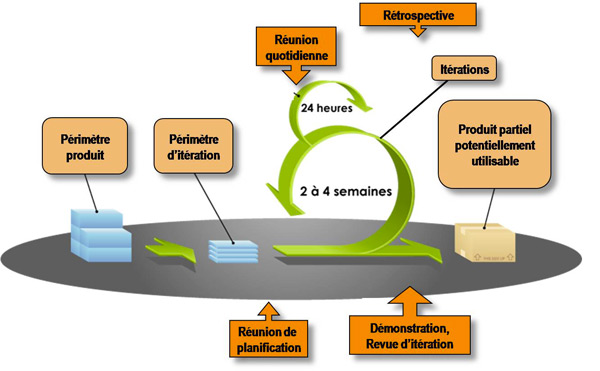
\includegraphics[width=17cm]{scrum-agiles.jpg}
\textit{Sources : \url{http://fr.wikipedia.org/wiki/Méthode_agile} et \url{http://fr.wikipedia.org/wiki/Scrum\_(méthode)}}
\subsection{Pourquoi ?}
Les méthodes agiles ont fait leur preuve dans leur efficacité et leur qualité de développement. De plus, Scrum permet un suivi et une transparence totale avec le client. Le découpage en sprint, itération assez courte, est adapté à notre projet puisqu'il se déroule sur une période relativement courte.

\section{Les livrables}
\begin{itemize}
\item Spécifications techniques des besoins
\item Analyse des risques
\item Cahier de recettes
\item Document d'architecture logicielle
\item Plan de développement détaillé
\item Politique de certification
\item Déclaration des pratiques de certification
\end{itemize}

\section{Organisation}
\begin{tabularx}{16cm}{|l|X|}
\hline
\textbf{Rôles} & \textbf{Qui ?}\\
\hline
Scrum Master / Chef de projet & Julien Legras\\
\hline
Représentant client & Jean-Baptiste Souchal\\

\hline
Architecte & Yves Nouafo\\

\hline
Testeur & Charles Ango\\
\hline
\end{tabularx}

\section{Dimensionnement}
\subsection{Stratégie}
Le développement de ce projet sera découpé en trois itérations (sprints). Chaque sprint durera quatre semaines avec une livraison le dernier jour du sprint. Pour chaque sprint sont prévues une période de correction de problèmes du sprint précédent ainsi qu'une période de tests.

\begin{paragraph}{Sprint 1}
Ce sprint consiste en le développement de :
\begin{itemize}
\item Serveur simple : la gestion des connexions à la base de données, des salons et la transmission de messages aux destinataires.
\item Client simple : la connexion et la déconnexion au serveur, l'envoi et la réception d'un message au serveur et l'interfaçage.
\end{itemize}
\end{paragraph}

\begin{paragraph}{Sprint 2}
Ce sprint consiste en le développement de :
\begin{itemize}
\item PKI : la certification de clef RSA, la vérification, l'envoi, la révocation et le stockage des certificats.
\item Client : demande et réception de certificat.
\item Cérémonie des clefs pour générer la clef privée de la PKI.
\end{itemize}
\end{paragraph}

\begin{paragraph}{Sprint 3}
Ce sprint consiste en le développement de :
\begin{itemize}
\item Serveur sécurisé : la gestion des salons privés, des clefs symétriques, l'authentification lors de la connexion et l'enregistrement d'un nouvel utilisateur.
\item Client sécurisé : la gestion des clefs, le chiffrement/déchiffrement, la vérification de l'intégrité et de l'authenticité des messages, la création/suppression/administration de salons privés.
\end{itemize}
\end{paragraph}

\subsection{Description des tâches}
Pour minimiser le risque de perte de sources, nous avons mis en place un dépôt git avant le début de la phase de développement (\url{http://github.com/legrajul/bavardage}). De plus, les phases d'apprentissage de nouvelles connaissances techniques sont incluses dans les tâches concernées.
~~\\

\begin{tabular}{|c|c|r|l|r|}
\hline
&&\textbf{Tâche} & \textbf{Description} & \textbf{Dépendances}\\
\hline
\multirow{11}{*}{\begin{sideways}\textbf{Sprint 1}\end{sideways}}&\multirow{5}{*}{\begin{sideways}\textbf{Serveur}\end{sideways}}&1& Gestion des connexions/déconnexions et BDD&\\
&& 2 & Salon d'accueil&1, 6\\
&& 3 & Création/suppression/gestion des salons publics & 1,6\\
&& 4 & Transmission des messages aux destinataires & 2\\
&& 5 & Envoi de messages privés non sécurisés& 1, 6\\
\cline{2-5}
&\multirow{6}{*}{\begin{sideways}\textbf{Client}\end{sideways}}& 6 & Connexion/déconnexion à un serveur avec pseudo&\\
&& 7 & Envoi/réception d'un message public/privé & 2\\
&& 8 &Envoi de demande de création de salon au serveur & 1, 6\\
&& 9 &Rejoindre/quitter un salon & 3, 8\\
&& 10.1 &Interface Gtk & \\
&& 10.2 &Interfaçage de la bibliothèque C en VAPI & 10.1\\
\hline

\multirow{8}{*}{\begin{sideways}\textbf{Sprint 2}\end{sideways}}&\textbf{Client}&1.1& Demande de certificat à la PKI &\\
&&1.2& Réception du certificat envoyé par la PKI & 1.1, 4\\
\cline{2-5}
&\multirow{6}{*}{\begin{sideways}\textbf{PKI}\end{sideways}}& 2 & Certification de clef RSA (AC)
 pseudo & 1.1, 3\\
&& 3 & Vérification des règles (RA) &\\
&& 4 & Envoi des certificats (AC) & 2\\
&& 5 & Stockage des certificats (AC)& 2\\
&& 6 & Permettre l'accès en lecture aux certificats (AC) & 5\\
&& 7 & Suppression d'un utilisateur & 5\\
\hline

\multirow{8}{*}{\begin{sideways}\textbf{Sprint 3}\end{sideways}}&\multirow{4}{*}{\begin{sideways}\textbf{Serveur S}\end{sideways}}&1& Gestion des salons privés & 3, 4\\
&&2& Gestion des clefs de chiffrement symétrique & 1, 6\\
&&3& Authentification lors de la connexion & \\
&&4& Enregistrement nouvel utilisateur & \\
\cline{2-5}
&\multirow{4}{*}{\begin{sideways}\textbf{Client S}\end{sideways}}& 5 & Chiffrement/déchiffrement des messages et gestion des clefs & 2, 8\\
&& 6 & Demande de suppression de compte & 3, 4\\
&& 7 & Création/suppression/administration de salon privé & 3, 4\\
&& 8 & Rejoindre/quitter un salon privé & 1, 7\\
\hline

\end{tabular}

\subsection{Évaluation des charges et répartition des tâches}
\begin{landscape}
\begin{tabularx}{20cm}{|c|r|r|r|r|r|X|c|c|}
\hline
&\textbf{Tâche} & \textbf{Complexité} & \textbf{Charge} & \textbf{Effectif} & \textbf{Délai} & \textbf{Qui ?} & \textbf{Début} & \textbf{Fin}\\

\hline
\multirow{11}{*}{\begin{sideways}\textbf{Sprint 1}\end{sideways}}& 1&4 &8 &2 &4 & Ismael -- Yves & 21/01/2013 & 24/01/2013\\
\cline{2-9}
& 2& 2& 6& 2& 3& Yves -- Jean-Baptiste& 25/01/2013 & 29/01/2013\\
\cline{2-9}
& 3& 3& 6& 2& 3& Ismael -- Julien& 26/01/2013& 28/01/2013\\
\cline{2-9}
& 4& 3& 3& 1& 3& Jean-Baptiste& 30/01/2013& 01/02/2013\\
\cline{2-9}
& 5& 2& 3& 1& 3& Charles& 31/01/2013& 04/02/2013\\
\cline{2-9}
& 6& 2& 3& 1& 3& Jean-Baptiste& 21/01/2013& 24/01/2013\\
\cline{2-9}
& 7& 2& 3& 1& 3& Yves& 30/01/2013& 01/02/2013\\
\cline{2-9}
& 8& 2& 3& 1& 3& Charles& 26/01/2013& 28/01/2013\\
\cline{2-9}
& 9& 2& 3& 1& 3& Ismael& 31/01/2013& 04/02/2013\\
\cline{2-9}
& 10.1& 6& 10& 2& 5&Julien -- Charles& 21/01/2013& 25/01/2013\\
\cline{2-9}
& 10.2& 4& 8& 2& 4& Julien& 04/02/2013& 07/02/2013\\

\hline
\multirow{8}{*}{\begin{sideways}\textbf{Sprint 2}\end{sideways}}& 1.1& 2& 8& 2& 4& Ismael -- Yves& 18/02/2013& 21/02/2013\\
\cline{2-9}
& 1.2& 2& 3& 1& 3& Ismael & 04/03/2013& 06/03/2013\\
\cline{2-9}
& 2& 3& 6& 2& 3& Charles -- Ismael& 22/02/2013& 26/02/2013\\
\cline{2-9}
& 3& 3& 8& 2& 4& Jean-Baptiste -- Julien& 18/02/2013& 21/02/2013\\
\cline{2-9}
& 4& 3& 6& 2& 3& Charles -- Julien& 27/02/2013&01/03/2013\\
\cline{2-9}
& 5& 3& 6& 2& 3& Jean-Baptiste -- Yves& 27/02/2013&01/03/2013\\
\cline{2-9}
& 6& 3& 6& 2& 3& Charles -- Julien& 04/03/2013&06/03/2013\\
\cline{2-9}
& 7& 2& 6& 2& 3& Jean-Baptiste -- Yves& 04/03/2013&06/03/2013\\

\hline
\multirow{8}{*}{\begin{sideways}\textbf{Sprint 3}\end{sideways}}& 1& 4& 8& 2& 4& Julien -- Jean-Baptiste& 22/03/2013& 27/03/2013\\
\cline{2-9}
& 2& 4& 6& 2& 3& Ismael -- Yves& 27/03/2013& 29/03/2013\\
\cline{2-9}
& 3& 4& 8& 2& 4& Jean-Baptiste -- Charles& 18/03/2013& 21/03/2013\\
\cline{2-9}
& 4& 4& 8& 2& 4& Ismael -- Julien& 18/03/2013& 21/03/2013\\
\cline{2-9}
& 5& 2& 8& 2& 4& Jean-Baptiste -- Julien& 01/04/2013& 04/04/2013\\
\cline{2-9}
& 6& 4& 3& 1& 3& Yves& 22/03/2013& 26/03/2013\\
\cline{2-9}
& 7& 2& 4& 2& 2& Charles -- Ismael& 22/03/2013& 25/03/2013\\
\cline{2-9}
& 8& 4& 4& 2& 2& Charles -- Julien& 28/03/2013& 29/03/2013\\

\hline


\end{tabularx}
\end{landscape}


\begin{landscape}
\protected\def\zzz{\ {\pgfcalendarjuliantodate{\numexpr\startdate\relax}{\year}{\month}{\day}\day/\month\global\advance\startdate1}}
\begin{tikzpicture}[x = 0.5cm]
\begin{ganttchart}[vgrid, bar top shift=0., bar height=1, y unit chart=0.5cm, x unit=1.5cm,inline]{14}
\gantttitle{Sprint 1 : Serveur et client de chat }{14}\\
\gantttitlelist[title list options={var=\y, evaluate=\y as \x using "\zzz"}]{1,...,14}{1}\\

\ganttbar[bar/.style={fill=green!50}]{10.1 (CA, JL)}{1}{5}
\ganttbar[bar/.style={fill=green!50}]{10.2 (JL)}{11}{12}\\
\ganttbar{1 (IK, YN)}{1}{5}\\
\ganttbar[bar/.style={fill=green!50}]{6 (JBS)}{1}{3}\\

\ganttbar{2 (YN,JBS)}{8}{10}\\
\ganttbar{3 (IK,JL)}{8}{10}\\
\ganttbar[bar/.style={fill=green!50}]{8 (CA)}{8}{10}\\
\ganttbar{4 (JBS)}{11}{12}\\
\ganttbar[bar/.style={fill=green!50}]{7 (YN)}{11}{12}\\
\ganttbar{5 (CA)}{11}{12}\\
\ganttbar[bar/.style={fill=green!50}]{9 (IK)}{11}{12}

\end{ganttchart}
\end{tikzpicture}
\\

\begin{tikzpicture}[x = 0.5cm]
\begin{ganttchart}[vgrid, bar top shift=0., bar height=1, y unit chart=0.5cm, x unit=1.5cm,inline]{14}
\gantttitlelist[title list options={var=\y, evaluate=\y as \x using "\zzz"}]{1,...,14}{1}\\
\ganttbar[bar/.style={fill=green!50}]{10.2 (JL)}{1}{3}\\
\\
\\
\\
\\
\ganttbar{4 (JBS)}{1}{1}\\
\ganttbar[bar/.style={fill=green!50}]{7 (YN)}{1}{1}\\
\ganttbar{5 (CA)}{1}{1}\\
\ganttbar[bar/.style={fill=green!50}]{9 (IK)}{1}{1}\\
\ganttbar[bar/.style={fill=red!50}]{Tests}{2}{5}
\ganttbar[bar/.style={fill=red!50}]{Tests}{8}{12}
\end{ganttchart}
\end{tikzpicture}

\newpage

\begin{tikzpicture}
\begin{ganttchart}[vgrid, bar top shift=0., bar height=1, y unit chart=0.5cm, x unit=1.5cm,inline]{14}
\gantttitle{Sprint 2 : Certificats}{14}\\
\gantttitlelist[title list options={var=\y, evaluate=\y as \x using "\zzz"}]{1,...,14}{1}\\
\ganttbar[bar/.style={fill=green!50}]{1.1 (IK, YN)}{1}{4}\\
\ganttbar[bar/.style={fill=yellow!50}]{3 (JL, JBS)}{1}{4}\\
\ganttbar[bar/.style={fill=yellow!50}]{2 (CA,IK)}{5}{5}
\ganttbar[bar/.style={fill=yellow!50}]{2 (CA,IK)}{8}{9}\\

\ganttbar[bar/.style={fill=yellow!50}]{4 (CA, JL)}{10}{12}\\
\ganttbar[bar/.style={fill=yellow!50}]{5 (YN, JBS)}{10}{12}\\

\end{ganttchart}
\end{tikzpicture}
\\

\begin{tikzpicture}
\begin{ganttchart}[vgrid, bar top shift=0., bar height=1, y unit chart=0.5cm, x unit=1.5cm,inline]{14}

\gantttitlelist[title list options={var=\y, evaluate=\y as \x using "\zzz"}]{1,...,14}{1}\\
\ganttbar[bar/.style={fill=green!50}]{1.2 (IK)}{1}{3}\\
\\
\\
\\
\\
\ganttbar[bar/.style={fill=yellow!50}]{6 (YN)}{1}{3}\\
\ganttbar[bar/.style={fill=yellow!50}]{7 (CA, IK)}{1}{3}\\
\ganttbar[bar/.style={fill=red!50}]{Tests}{8}{12}
\ganttbar[bar/.style={fill=red!50}]{Correction bugs sprint 1}{1}{5}
\end{ganttchart}
\end{tikzpicture}



\newpage



\begin{tikzpicture}
\begin{ganttchart}[vgrid, bar top shift=0., bar height=1, y unit chart=0.5cm, x unit=1.5cm,inline]{14}
\gantttitle{Sprint 3 : Serveur et client de chat sécurisés}{14}\\
\gantttitlelist[title list options={var=\y, evaluate=\y as \x using "\zzz"}]{1,...,14}{1}\\
\ganttbar{Apprentissage SSL}{1}{5}\\
\ganttbar{3 (CA, IK)}{8}{12}\\
\ganttbar{4 (YN, JBS)}{8}{12}\\



\ganttbar[bar/.style={fill=red!50}]{Correction bugs sprint 2}{1}{5}
\ganttbar[bar/.style={fill=red!50}]{Configuration serveur EJBCA (JL)}{8}{12}

\end{ganttchart}
\end{tikzpicture}

\begin{tikzpicture}
\begin{ganttchart}[vgrid, bar top shift=0., bar height=1, y unit chart=0.5cm, x unit=1.5cm,inline]{14}
\gantttitlelist[title list options={var=\y, evaluate=\y as \x using "\zzz"}]{1,...,14}{1}\\
\ganttbar{3 (CA, IK)}{1}{5}\\
\ganttbar{4 (YN, JBS)}{1}{5}\\
\ganttbar[bar/.style={fill=red!50}]{Configuration serveur EJBCA (JL)}{1}{5}

\ganttbar{Apprentissage EVP}{8}{12}\\
\ganttbar[bar/.style={fill=green!50}]{9 (JL)}{8}{10}\\

\end{ganttchart}
\end{tikzpicture}

\begin{tikzpicture}
\begin{ganttchart}[vgrid, bar top shift=0., bar height=1, y unit chart=0.5cm, x unit=1.5cm,inline]{14}
\gantttitlelist[title list options={var=\y, evaluate=\y as \x using "\zzz"}]{1,...,14}{1}\\

\ganttbar[bar/.style={fill=green!50}]{5 (CA)}{8}{11}\\

\ganttbar{1 (JL, JBS)}{8}{11}\\

\ganttbar[bar/.style={fill=green!50}]{7 (C, I)}{12}{12}\\

\ganttbar{2 (IK, YN)}{8}{11}\\



\end{ganttchart}
\end{tikzpicture}


\begin{tikzpicture}
\begin{ganttchart}[vgrid, bar top shift=0., bar height=1, y unit chart=0.5cm, x unit=1.5cm,inline]{7}
\gantttitlelist[title list options={var=\y, evaluate=\y as \x using "\zzz"}]{1,...,7}{1}\\

\ganttbar[bar/.style={fill=green!50}]{7 (C, I)}{1}{1}\\
\ganttbar[bar/.style={fill=green!50}]{8 (C, J)}{2}{3}\\
\ganttbar[bar/.style={fill=green!50}]{6 (YN, JBS)}{1}{2}\\

\ganttbar[bar/.style={fill=red!50}]{Tests}{1}{5}

\end{ganttchart}
\end{tikzpicture}
\end{landscape}


\section{Suivi}
\subsection{Gestion électronique des documents}
Pour partager les documents, un dépôt git a été mis en place sur Github à l'adresse : 

\href{url: https://github.com/legrajul/bavardage-doc}{https://github.com/legrajul/bavardage-doc}

\subsection{Réunions}
\subsubsection{Réunions avec le client}
\begin{paragraph}{Réunion n\degree1 -- 07/11/2012}
Première présentation du projet par le client.
\end{paragraph}

\begin{paragraph}{Réunion n\degree2 --14/11/2012}
Différentes questions ont été posées pour pouvoir réaliser la STB :
\begin{enumerate}
\item Lors de la connexion, l'utilisateur se retrouve-t-il dans un salon d'accueil ?
\item [] $\hookrightarrow$ Oui, les messages échangés sur ce salon ne seront pas chiffrés.

\item Il y a-t-il des salons publics ?
\item [] $\hookrightarrow$ Oui, comme pour le salon d'accueil, les messages échangés sur ce salon ne seront pas chiffrés.
\item [] $\hookrightarrow$ Pas besoin de s'enregistrer pour y accéder et y bavarder.

\item Que se passe-t-il lorsque le créateur d'un salon se déconnecte ?
\item [] $\hookrightarrow$ Fermeture du salon avec avertissement.

\item Qui créé un compte sécurisé ?
\item [] $\hookrightarrow$ L'autorité de certification, elle est automatique et applique une politique de certification.

\item Quelles sont les attentes au niveau de l'interface graphique ?
\item [] $\hookrightarrow$ Elle doit rester simple et il doit également être possible d'utiliser le logiciel en lignes de commandes.

\item  Quelles sont les qualités attendues ?
\begin{itemize}
\item le niveau de crypto ne doit pas impacter les performances;
\item l'ajout et la suppression d'un utilisateur doit être rapide pour ne pas perdre de message.
\end{itemize}

\item Quelles sont les exigences opérationnelles ?
\begin{itemize}
\item création d'un salon privé (avec la liste des personnes autorisées à s'y connecter);
\item ajout et suppression d'une nouvelle personne dans un groupe privé;
\item diffusion des clefs de chiffrement;
\item communication multi--salons.
\end{itemize}

\item Quelles sont les exigences de réalisation ?
\begin{itemize}
\item documentation rédigée en \LaTeX;
\item utilisation d'OpenSSL;
\item utilisation de tinyca pour créer l'autorité de certification.
\end{itemize}

\item Quelles sont les exigences au de l'interface de communication ?
\item [] $\hookrightarrow$ Le serveur sécurisé doit pouvoir s'adapter à d'autres protocoles, il doit être indépendant du serveur de bavardage.

\item Autorité de certification
\item [] $\hookrightarrow$ fournit des certificats = une clef publique + identité + date d'expiration + \dots

\item Politique de certification
\item [] $\hookrightarrow$ Qui ?
\item [] $\hookrightarrow$ Comment se fait la vérification d'identité ?
\item [] $\hookrightarrow$ Comment se fait la révocation ?
\item [] $\hookrightarrow$ \dots
\end{enumerate}
\end{paragraph}

\begin{paragraph}{Réunion n\degree3 -- 21/11/2012}
Précisions apportées sur des cas d'utilisation :
\begin{itemize}
\item Lorsqu'un utilisateur est invité, il y a changement de clef seulement quand il rejoint le salon.
\item Paramétrage de compte sécurisé pour choisir s'il peut envoyer/recevoir des messages privés non sécurisés avec un utilisateur non authentifié.
\item Comment effectuer une demande de certificat ?
\item [] $\hookrightarrow$  page d'administration accessible par une ou plusieurs personnes pour valider le certificat ;
\item [] $\hookrightarrow$ il faut que l'utilisateur génère sa propre paire de clefs publique/privée puis l'AC certifie cette paire de clefs.
\item La révocation d'un certificat est assurée par l'AC et est demandée soit par un administrateur de salon, soit pas le propriétaire du certificat.
\end{itemize}
Présentation d'une politique de certification (avec la PKI).
\end{paragraph}

\begin{paragraph}{Réunion n\degree4 -- 05/12/2012}Réunion après premier retour du client sur la STB
\end{paragraph}

\begin{paragraph}{Réunion n\degree5 -- 12/12/2012}Réunion après deuxième retour du client sur la STB et présentation des schémas du DAL.
\end{paragraph}

\begin{paragraph}{Réunion n\degree6 -- 19/12/2012}Présentation du DAL version électronique et du CdR. Présentation de EJBCA (Enterprise Java Bean Certificate Authority) par le client.
\end{paragraph}

\subsubsection{Réunions TD}
\begin{paragraph}{TD n\degree1 -- 09/11/2012}
Première réunion avec le responsable de gestion de projet, présentation des différents documents à fournir et des différents rôles à attribuer.
\end{paragraph}

\begin{paragraph}{TD n\degree2 -- 16/11/2012}
Deuxième TD de GDP avec à l'ordre du jour la rédaction de la STB avec l'aide du chargé de TD.
\end{paragraph}

\begin{paragraph}{TD n\degree3 -- 23/11/2012}
Troisième TD de GDP avec à l'ordre du jour la rédaction du cahier de recette, du document d'architecture du logiciel et de l'analyse des risques avec l'aide du chargé de TD.
\end{paragraph}

\begin{paragraph}{TD n\degree4 -- 30/11/2012}
Quatrième TD de GDP avec à l'ordre du jour la présentation au chargé de TD du cahier de recette, du document d'architecture du logiciel et de l'analyse des risques qui ont été commencés et présentation du document de planning de développement par le chargé de TD.
\end{paragraph}

\begin{paragraph}{TD n\degree5 -- 07/12/2012}
Cinquième TD de GDP avec à l'ordre du jour la présentation au chargé de TD de l'avancement des documents et présentation de la méthode pour faire un plan de développement par le chargé de TD.
\end{paragraph}

\subsubsection{Réunions de groupe}
Il y a eu plusieurs points rapides faits tout au long de l'élaboration des documents mais leur courte durée ne permet pas de les qualifier de réunions.

\begin{paragraph}{07/11/2012}
Débriefing après la première réunion avec le client.
\end{paragraph}

\begin{paragraph}{26/11/2012}
Présentation de l'outil Git par Julien Legras.
\end{paragraph}

\begin{paragraph}{12/12/2012}
Évaluation des charges des tâches.
\end{paragraph}

\begin{paragraph}{17/12/2012}
Élaboration des diagrammes de Gantt et répartition des tâches.
\end{paragraph}

\subsubsection{Réunions pendant le développement}
Une réunion avec le client sera faite quelques jours avant la livraison pour lui montrer ce qui sera livré ainsi qu'une autre quelques jours après la livraison pour le client puisse faire un retour sur les éventuels bugs et/ou améliorations à apporter.

\begin{paragraph}{Sprint 1 -- semaine 1 -- 21/01/2013}
L’ordre du jour de la réunion était : lancement du projet, coordination des tâches par rapport au plan de développement.

Selon le plan de développement établi lors des séances de travaux pratiques de gestion de projet, le projet de chat sécurisé devait être lancé le 21 Janvier 2013. Les tâches de la semaine : 1, 6, 10.1
\end{paragraph}

\begin{paragraph}{Sprint 1 -- semaine 2 -- 28/01/2013}
L’ordre du jour de la réunion était : coordination des tâches par rapport au plan de développement.

Les tâches de la semaine : 2, 3, 4, 5, 7, 8, 9
\end{paragraph}

\begin{paragraph}{Sprint 1 -- semaine 3 -- 04/02/2013}
L’ordre du jour de la réunion était : coordination des tâches par rapport au plan de développement

Les tâches de la semaine : 4, 5, 7, 9, 10.2
\end{paragraph}

\begin{paragraph}{Sprint 1 -- semaine 4 -- 11/02/2013}
L’ordre du jour de la réunion était : coordination des tâches par rapport au plan de développement

Les tâches de la semaine : tests
\end{paragraph}

\begin{paragraph}{Sprint 2 -- semaine 1 -- 18/02/2013}
L’ordre du jour de la réunion était : coordination des tâches par rapport au plan de développement

Les tâches de la semaine : 1.1, 2, 3
\end{paragraph}

\begin{paragraph}{Sprint 2 -- semaine 2 -- 25/02/2013}
L’ordre du jour de la réunion était : coordination des tâches par rapport au plan de développement

Les tâches de la semaine : 2, 4, 5
\end{paragraph}

\begin{paragraph}{Sprint 2 -- semaine 3 -- 04/03/2013}
L’ordre du jour de la réunion était : coordination des tâches par rapport au plan de développement

Les tâches de la semaine : 1.2, 6, 7
\end{paragraph}

\begin{paragraph}{Sprint 2 -- semaine 4 -- 11/03/2013}
L’ordre du jour de la réunion était : coordination des tâches par rapport au plan de développement.

Les tâches de la semaine : tests
\end{paragraph}

\begin{paragraph}{Sprint 3 -- semaine 1 -- 18/03/2013}
L’ordre du jour de la réunion était : préparation aux tâches du plan de développement.

Les tâches de la semaine : apprentissage d'OpenSSL (connexions sécurisées SSL).
\end{paragraph}

\begin{paragraph}{Sprint 3 -- semaine 2 -- 25/03/2013}
L’ordre du jour de la réunion était : coordination des tâches par rapport au plan de développement.

Les tâches de la semaine : 3, 4, configuration serveur mis à disposition par la fac pour EJBCA.
\end{paragraph}

\begin{paragraph}{Sprint 3 -- semaine 3 -- 01/04/2013}
L’ordre du jour de la réunion était : coordination des tâches par rapport au plan de développement.

Les tâches de la semaine : 3, 4
\end{paragraph}

\begin{paragraph}{Sprint 3 -- semaine 4 -- 08/04/2013}
L’ordre du jour de la réunion était : coordination des tâches par rapport au plan de développement.

Les tâches de la semaine : interface partie sécurisée, apprentissage d'OpenSSL (chiffrement symétrique)
\end{paragraph}

\begin{paragraph}{Sprint 3 -- semaine 5 -- 23/04/2013}
L’ordre du jour de la réunion était : coordination des tâches par rapport au plan de développement.

Les tâches de la semaine : 1, 2, 5, 7, 8
\end{paragraph}

\end{document}